%%% lorem.tex --- 
%% 
%% Filename: lorem.tex
%% Description: 
%% Author: Ola Leifler
%% Maintainer: 
%% Created: Wed Nov 10 09:59:23 2010 (CET)
%% Version: $Id$
%% Version: 
%% Last-Updated: Wed Nov 10 09:59:47 2010 (CET)
%%           By: Ola Leifler
%%     Update #: 2
%% URL: 
%% Keywords: 
%% Compatibility: 
%% 
%%%%%%%%%%%%%%%%%%%%%%%%%%%%%%%%%%%%%%%%%%%%%%%%%%%%%%%%%%%%%%%%%%%%%%
%% 
%%% Commentary: 
%% 
%% 
%% 
%%%%%%%%%%%%%%%%%%%%%%%%%%%%%%%%%%%%%%%%%%%%%%%%%%%%%%%%%%%%%%%%%%%%%%
%% 
%%% Change log:
%% 
%% 
%% RCS $Log$
%%%%%%%%%%%%%%%%%%%%%%%%%%%%%%%%%%%%%%%%%%%%%%%%%%%%%%%%%%%%%%%%%%%%%%
%% 
%%% Code:

\chapter{Resultat}
\label{cha:results}

Resultatet av Entropi-estimeringen, Huffman-kodningen och LZW-kodningen presenteras i figur \ref{fig:results}. För varje fil, som presenteras i raderna, ser vi entropin, H(Xi), H(Xi|Xi-1) och H(Xi|Xi-1, Xi-2). Vi ser även vilken takt (rate) vi kan koda med Huffman-kodning och LZW-kodning. Vi ser även hur mycket plats vi sparar med Huffman-kodning och LZW-kodning för respektive fil.
\begin{figure}
  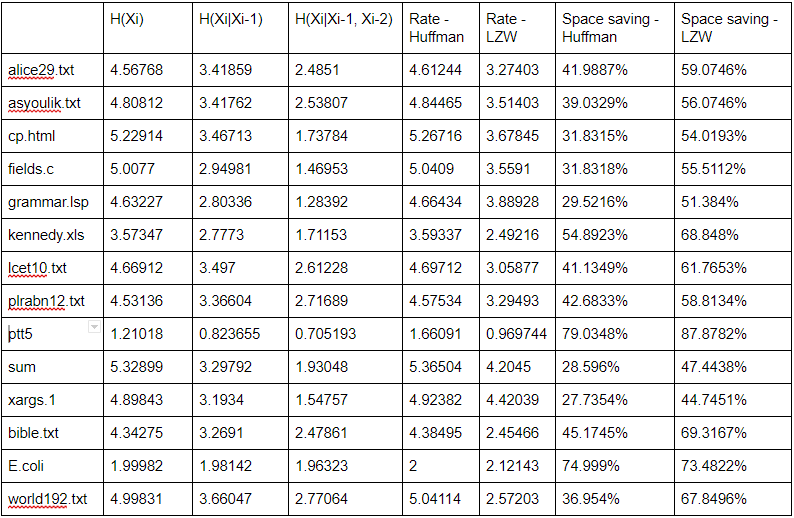
\includegraphics[width=\linewidth]{results.png}
  \caption{Resultat av entropi-estimeringen, Huffman-kodningen och LZW-kodningen.}
  \label{fig:results}
\end{figure}

Att komprimera en fil med Huffman-kodning lyckades bra. Låt oss säga att vi har en fil med innehållet "huffman". Den komprimerade Huffman-filen ser vi i figur \ref{fig:huffmanresults}. I filen ser vi den bitsekvens som filen har komprimerats till. Vi ser även den så kallade headern, den representerar frekvenstabellen som även nämndes i teori- och metodavsnittet. Vi ser till exempel först 97:1, vilket representerar ASCII-tecken 97 och efter kolonet ser vi många 97 det finns i filen, det vill säga 1. ASCII-tecken 97 motsvarar symbolen a. Vi ser sedan att det finns två stycken 102, vilket motsvarar symbolen f. Resultatet av detta exempel på Huffman-kodning blir att den har komprimerats från 8*7 = 56 bitar till 36*8 + 18 = 306 bitar. Detta är såklart ingen komprimering överhuvudtaget, filen har blivit större, varför det blivit så diskuteras senare. Vid avkomprimering av Huffman-filen läses frekvenstabellen in först, för att sedan bygga upp Huffman-trädet och läsa av bit för bit i Huffman-filen. Detta fungerar utmärkt.
\begin{figure}
  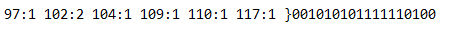
\includegraphics[width=\linewidth]{Huffman-result.png}
  \caption{En Huffman-fil som komprimerat en fil med innehållet "huffman".}
  \label{fig:huffmanresults}
\end{figure}

Att komprimera en fil med LZW-kodning lyckades bra. Låt oss säga att vi har en fil med innehållet "huffman". Den komprimerade LZW-filen ser vi i figur \ref{fig:lzwresults}. I filen ser vi den bitsekvens som filen har komprimerats till. Resultatet av detta exempel på LZW-kodning blir att den har komprimerats från 8*7 = 56 bitar till 62 bitar. Detta är inte heller någon komprimering, utan filen har blivit större, varför det blivit så diskuteras senare. Att avkomprimera LZW-filen görs genom att läsa av bitsekvensen, vilket fungerar utmärkt.

\begin{figure}
  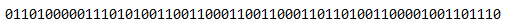
\includegraphics[width=\linewidth]{LZW-result.png}
  \caption{En LZW-fil som komprimerat en fil med innehållet "huffman".}
  \label{fig:lzwresults}
\end{figure}

%%%%%%%%%%%%%%%%%%%%%%%%%%%%%%%%%%%%%%%%%%%%%%%%%%%%%%%%%%%%%%%%%%%%%%
%%% lorem.tex ends here

%%% Local Variables: 
%%% mode: latex
%%% TeX-master: "demothesis"
%%% End: 
